\documentclass[aoas]{imsart}
%% LaTeX 2e style file for the processing of LaTeX2e files
%% of the following IMS/BS journals:
%%
%% - The Annals of Probability
%% - The Annals of Applied Probability
%% - The Annals of Statistics
%% - The Annals of Applied Statistics
%% - Statistical Science
%% - Probability Surveys
%% - Statistics Surveys
%% - Electronic Journal of Statistics
%% - Bernoulli
%% - Annales de l'Institut Henri Poincar\'e - Probabilit\'es et Statistiques
%% - Brazilian Journal of Probability and Statistics
%% - Bayesian Analysis
%%
%% - Institute of Mathematical Statistics, U.S.A.
%% - Bernoulli Society
%% - Institut Henry Poincare
%% - Brazilian Statistical Association
%% - International Society for Bayesian Analysis
%%
%% Macros written by Vytas Statulevicius, VTeX, Lithuania
%% Maintained by TeX group members, VTeX, Lithuania
%% for Institute of Mathematical Statistics, U.S.A.
%% Please submit bugs or your comments to latex-support@vtex.lt
%%
%% The original distribution is located at:
%% https://www.e-publications.org/ims/support

\RequirePackage{amsthm,amsmath,amsfonts,amssymb}
\RequirePackage[authoryear]{natbib}
\RequirePackage[colorlinks,citecolor=blue,urlcolor=blue]{hyperref}
\RequirePackage{graphicx}

% Added package
\usepackage[T1]{fontenc}
\usepackage[english]{babel}


% tightlist command for lists without linebreak
\providecommand{\tightlist}{%
  \setlength{\itemsep}{0pt}\setlength{\parskip}{0pt}}



% Garantees bookdown compilation
%\usepackage{lmodern}

\makeatletter
\def\maxwidth{\ifdim\Gin@nat@width>\linewidth\linewidth\else\Gin@nat@width\fi}
\def\maxheight{\ifdim\Gin@nat@height>\textheight\textheight\else\Gin@nat@height\fi}
\makeatother
% Scale images if necessary, so that they will not overflow the page
% margins by default, and it is still possible to overwrite the defaults
% using explicit options in \includegraphics[width, height, ...]{}
\setkeys{Gin}{width=\maxwidth,height=\maxheight,keepaspectratio}
% Set default figure placement to htbp
\makeatletter
\def\fps@figure{htbp}
\makeatother
\setlength{\emergencystretch}{3em} % prevent overfull lines

% alternative version to the shaded problem
\makeatletter
\@ifundefined{Shaded}{
}{\renewenvironment{Shaded}{\begin{kframe}}{\end{kframe}}}
\makeatother

\startlocaldefs
%%%%%%%%%%%%%%%%%%%%%%%%%%%%%%%%%%%%%%%%%%%%%
%                                          %%
% Uncomment next line to change            %%
% the type of equation numbering           %%
%                                          %%
%%%%%%%%%%%%%%%%%%%%%%%%%%%%%%%%%%%%%%%%%%%%%
\numberwithin{equation}{section}
%%%%%%%%%%%%%%%%%%%%%%%%%%%%%%%%%%%%%%%%%%%%%
%                                          %%
% For Axiom, Claim, Corollary, Hypothezis, %%
% Lemma, Theorem, Proposition              %%
% use \theoremstyle{plain}                 %%
%                                          %%
%%%%%%%%%%%%%%%%%%%%%%%%%%%%%%%%%%%%%%%%%%%%%
\theoremstyle{plain}
\newtheorem{axiom}{Axiom}
\newtheorem{claim}[axiom]{Claim}
\newtheorem{theorem}{Theorem}[section]
\newtheorem{lemma}[theorem]{Lemma}
%%%%%%%%%%%%%%%%%%%%%%%%%%%%%%%%%%%%%%%%%%%%%
%                                          %%
% For Assumption, Definition, Example,     %%
% Notation, Property, Remark, Fact         %%
% use \theoremstyle{remark}                %%
%                                          %%
%%%%%%%%%%%%%%%%%%%%%%%%%%%%%%%%%%%%%%%%%%%%%
\theoremstyle{remark}
\newtheorem{definition}[theorem]{Definition}
\newtheorem*{example}{Example}
\newtheorem*{fact}{Fact}
%%%%%%%%%%%%%%%%%%%%%%%%%%%%%%%%%%%%%%%%%%%%%
% Please put your definitions here:        %%
%%%%%%%%%%%%%%%%%%%%%%%%%%%%%%%%%%%%%%%%%%%%%
\endlocaldefs

% pandoc header
\usepackage{listings}
\usepackage{xcolor}
\usepackage{float}
\floatplacement{figure}{H}
% pandoc header
\usepackage{booktabs}
\usepackage{longtable}
\usepackage{array}
\usepackage{multirow}
\usepackage{wrapfig}
\usepackage{float}
\usepackage{colortbl}
\usepackage{pdflscape}
\usepackage{tabu}
\usepackage{threeparttable}
\usepackage{threeparttablex}
\usepackage[normalem]{ulem}
\usepackage{makecell}
\usepackage{xcolor}

\begin{document}



\begin{frontmatter}
%%%%%%%%%%%%%%%%%%%%%%%%%%%%%%%%%%%%%%%%%%%%%%
%%                                          %%
%% Enter the title of your article here     %%
%%                                          %%
%%%%%%%%%%%%%%%%%%%%%%%%%%%%%%%%%%%%%%%%%%%%%%
\title{STAT 444 FINAL PROJECT PAPER}
%\title{A sample article title with some additional note\thanksref{T1}}
\runtitle{}
%\thankstext{T1}{A sample of additional note to the title.}



\begin{aug}
%%%%%%%%%%%%%%%%%%%%%%%%%%%%%%%%%%%%%%%%%%%%%%
%%Only one address is permitted per author. %%
%%Only division, organization and e-mail is %%
%%included in the address.                  %%
%%Additional information can be included in %%
%%the Acknowledgments section if necessary. %%
%%%%%%%%%%%%%%%%%%%%%%%%%%%%%%%%%%%%%%%%%%%%%%

%% Example:
%%\author[A]{\fnms{First} \snm{Author}\ead[label=e1]{first@somewhere.com}},
%%\author[B]{\fnms{Second} \snm{Author}\ead[label=e2,mark]{second@somewhere.com}}
%%\and
%%\author[B]{\fnms{Third} \snm{Author}\ead[label=e3,mark]{third@somewhere.com}}

\author[A]{\fnms{Angelo} \snm{Carreon}
  \ead[label=e1, mark]{jaccarre@uwaterloo.ca}}
  

%%%%%%%%%%%%%%%%%%%%%%%%%%%%%%%%%%%%%%%%%%%%%%
%% Addresses                                %%
%%%%%%%%%%%%%%%%%%%%%%%%%%%%%%%%%%%%%%%%%%%%%%
%% Example:
%%\address[B]{Department,
%%University or Company Name,
%%\printead{e2,e3}}
\address[A]{Department of Statistics and Actuarial Science, University
of Waterloo,
  \printead{e1}}
\end{aug}

\begin{abstract}
This paper answers the question: which regression method best predicts
the prices of houses given their characteristics? To do this, four
different regression techniques were fitted to the Ames Housing dataset,
a popular collection of house sales that was prepared for an
end-of-semseter regression project. This dataset was processed to
address missing values, perform dimensionality reduction, and remove
outliers. A multiple linear regression, ridge regression, lasso
regression, and generalized additive model were then fitted to this
processed data and their root mean squared errors were compared using
cross-validation. It was found that a Generalized Additive model best
fit the data, due to the non-linear relationships present in the
covariates.
\end{abstract}


\begin{keyword}
\kwd{housing}
\kwd{advanced regression}
\end{keyword}

\end{frontmatter}


\newenvironment{kframe}{}{}

\hypertarget{introduction-to-our-chosen-dataset}{%
\section{Introduction to our chosen
dataset}\label{introduction-to-our-chosen-dataset}}

Our project aims to assess the feasibility of utilizing regression
techniques for interpolating and modeling housing prices. We have
selected a dataset of housing prices in Ames, Iowa, along with their
features from the \emph{Journal of Statistics Education}
\citep{cock2011amesdataset}. This dataset was prepared by Dean De Cock
for use as an end-of-semester regression project. His intent was to
provide data of substantial size (\(n=2930\)) with easy-to-understand
variables that are known to affect the final sale price such as build
date, lot size, and living space square footage. Applying this to
today's real estate market, we wish to answer the following question:
\emph{which regression method best predicts the prices of houses given
their characteristics}?

\hypertarget{exploratory-data-analysis}{%
\section{Exploratory Data Analysis}\label{exploratory-data-analysis}}

This dataset contains 2930 rows and 80 columns. There are 80 explanatory
variables, consisting of 23 nominal, 23 ordinal, 14 discrete, and 20
continuous variables. Several columns contain many missing values and
will be dropped before we begin fitting models. As highlighted in De
Cock's paper, several unusual outlier house sales exist in the data;
these will also be removed. There are no duplicate rows.

As seen in figure \ref{resp}, the distribution of \texttt{Sale\ Price}
is significantly right-skewed. The sale prices range from \$12,789 to
\$755,000 with a mean of \$180,796 and a standard deviation of
\$79,886.69. To achieve a more normal distribution, we can apply a log
transformation on the dependent variable, as seen below:

\begin{figure}
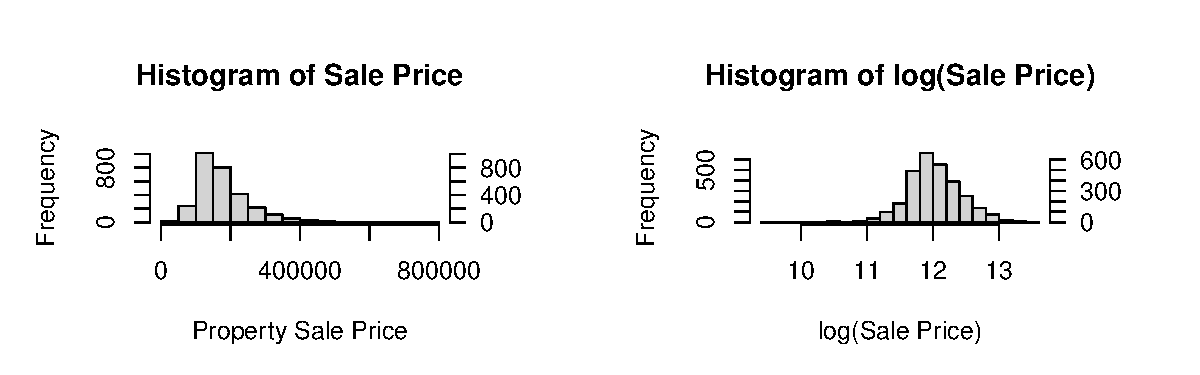
\includegraphics[trim={0 1cm 0 1cm},clip]{STAT-444-FINAL-PROJECT-PAPER_files/figure-latex/unnamed-chunk-3-1} \caption{Histograms of the response variable, Sale Price\label{resp}}\label{fig:unnamed-chunk-3}
\end{figure}

Some variables of interest are \texttt{Neighbourhood} and
\texttt{Lot.Area}, where we see in figure \ref{neighbourhood} to have
significant differences in the average property sale price. One way in
which these neighborhoods could differ is in the size of the lots of the
houses that reside there. Our team would need to consider variable
associations such as these to deal with collinearity.

\begin{figure}
\centering
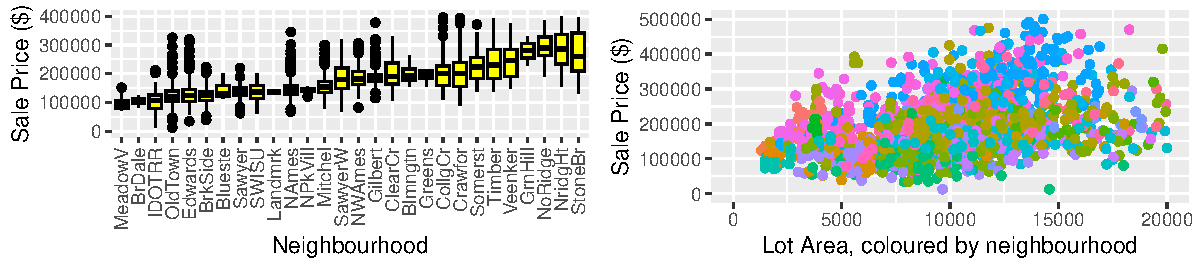
\includegraphics{STAT-444-FINAL-PROJECT-PAPER_files/figure-latex/unnamed-chunk-4-1.pdf}
\caption{Plots showing the distribution of final Sale Price across the
different Neighborhoods\label{neighbourhood}}
\end{figure}

\hypertarget{methods}{%
\section{Methods}\label{methods}}

There were three steps in the process of determining the most effective
regression model for predicting house prices: data preprocessing, model
fitting, and cross-validation. Preprocessing was used to clean the data,
upon which models were fitted and evaluated against each other using a
cross-validation scheme.

\hypertarget{data-preprocessing-and-dimensionality-reduction}{%
\subsection{Data Preprocessing and Dimensionality
Reduction}\label{data-preprocessing-and-dimensionality-reduction}}

Below is the pipeline we used to process the data:

\begin{figure}
\centering
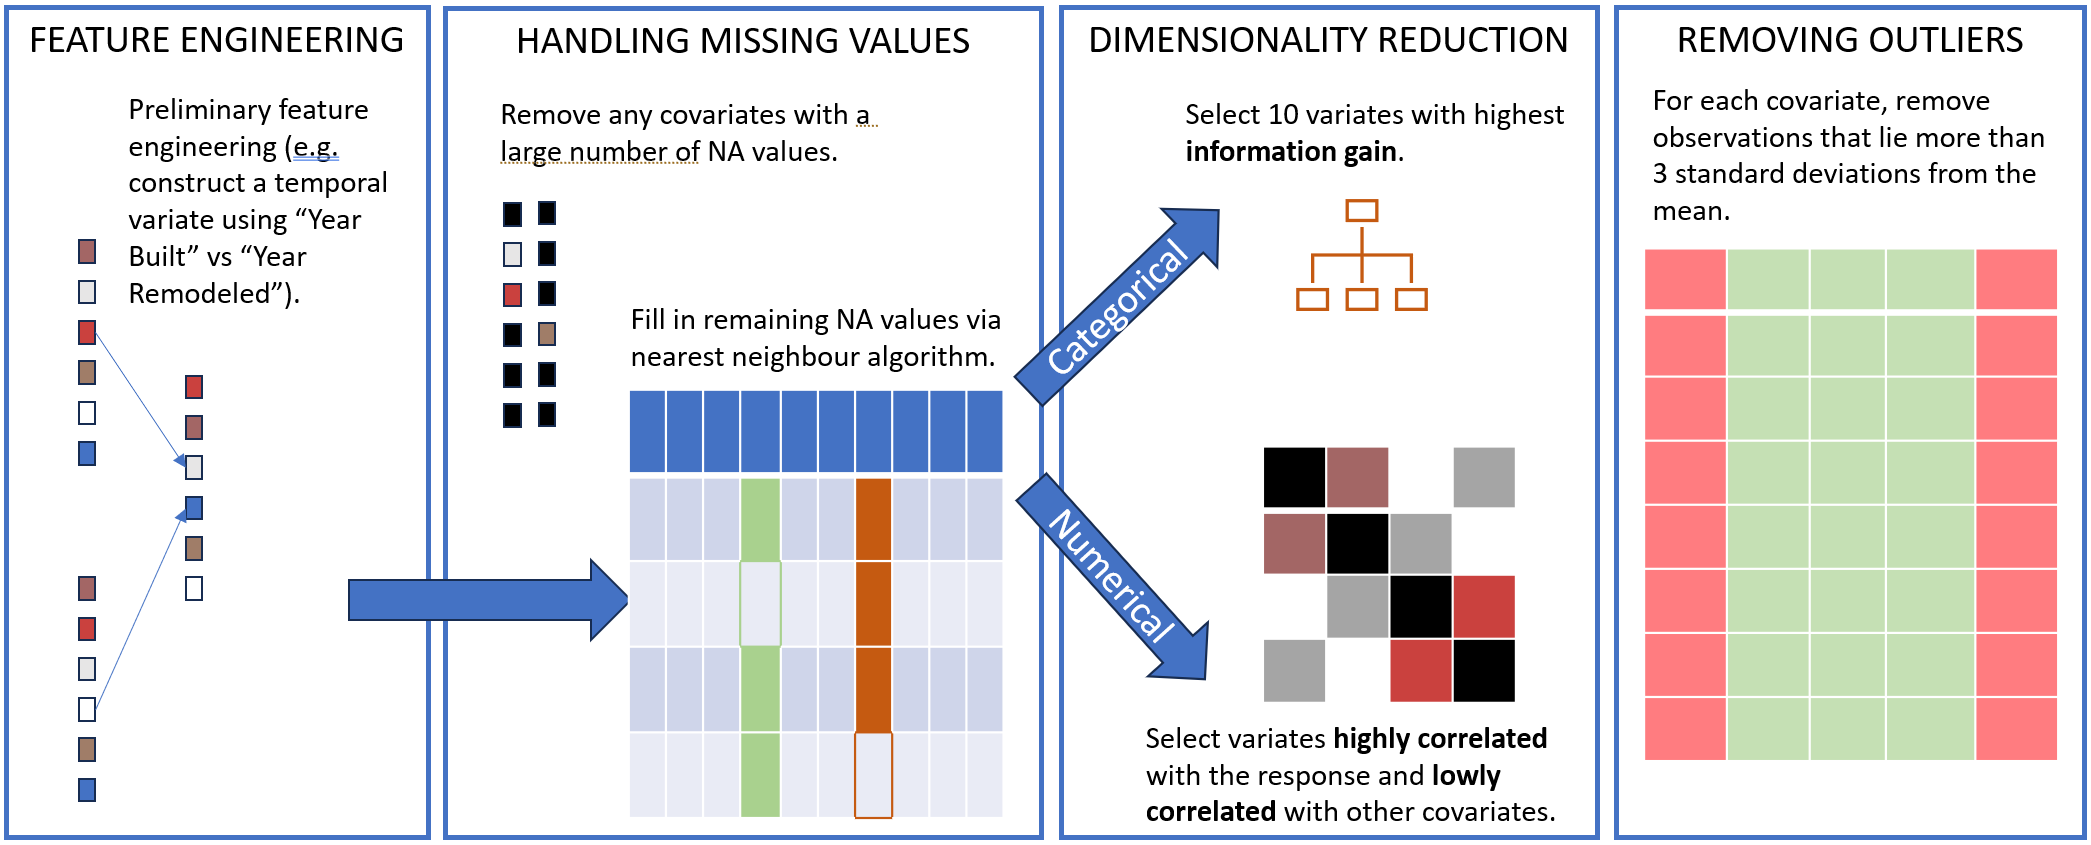
\includegraphics[width=5.20833in,height=\textheight]{images/EDA_PREPROCESSING.png}
\caption{Ames Housing data processing pipeline}
\end{figure}

\begin{itemize}
\item
  First, we did some feature engineering in order to differentiate the
  \texttt{Year.Built} and \texttt{Year.Remodeled} covariates. We
  replaced the \texttt{Year.Remodeled} covariate with the difference in
  years between renovation and construction, so that the rest of our
  processing steps can correctly differentiate between these two
  covariates.
\item
  Then, we addressed missing values in the data by removing covariates
  that had majority null values. A nearest neighbor algorithm was used
  on the remaining covariates to impute the remaining missing values.
\item
  Next, we employed dimensionality reduction, reducing the number of
  covariates to 19.

  \begin{itemize}
  \tightlist
  \item
    For categorical variables, we selected the top 10 that had the
    highest information gain. The specific calculation of this score is
    defined in \citet{quinlaninduction}. In summary, information gain
    measures the reduction in uncertainty about the target variable when
    the data is split based on a specific feature, helping decision tree
    algorithms identify the most valuable features for prediction.
  \item
    For numeric variables, one covariate from each group of highly
    correlated features was kept, and any covariates that showed weak
    linear relationships were removed.
  \end{itemize}
\item
  In order for our models to correctly interpret the categorical
  variables, their levels were factorized and converted into numeric
  values. Some categorical variables were ratings ranging from poor
  \(\to\) excellent. These were converted to ordinal covariates, whose
  values increase as the rating increases.
\item
  Lastly, to address outliers, we removed any observations that had a
  covariate whose values lie more than 3 standard deviations from the
  mean.
\end{itemize}

After the data preprocessing step, we were left with \(19\) covariates:
\(5\) nominal, \(5\) ordinal, \(5\) discrete, and \(4\) continuous.
Before any models were fit, the data was partitioned into training and
testing splits at an 80:20 ratio.

\hypertarget{model-fitting}{%
\subsection{Model Fitting}\label{model-fitting}}

Four regression techniques were compared in our analysis: Multiple
Linear Regression, Ridge Regression, Lasso Regression, and a Generalized
Additive Model.

\begin{itemize}
\tightlist
\item
  The MLR model was fit using R's built-in \texttt{lm} object, which
  solves Ordinary Least Squares:
\end{itemize}

\[
\min_{\beta} \sum_{i=1}^N(y_i - \beta_0 - \sum_{j=1}^px_{ij}\beta_j)^2
\]

\begin{itemize}
\tightlist
\item
  Both the Ridge and Lasso regression models were fit using the
  \texttt{glmnet} package, which uses cyclical coordinate descent to
  efficiently solve
\end{itemize}

\[
\min_{\beta}\frac{1}{2N}\sum_{i=1}^N(y_i-x_i^T\beta)^2 + \lambda[(1-\alpha)||\beta||_2^2/2 + \alpha||\beta||_1]
\]

where \(0 \leq \alpha \leq 1\) is the elastic net penalty and
\(\lambda \geq 0\) controls its strength \citep{JSSv033i01}.
\(\alpha=0\) was used to obtain a ridge penalty, and \(\alpha=1\) was
used to obtain lasso penalty. For both ridge and lasso regression, the
optimal \(\lambda\) value was chosen to minimize mean-squared error via
grid search under a 10-fold cross-validation scheme. An example of the
output of the hyperparameter fit of \(\lambda\) for both ridge and lasso
regression using the training set is below:

\begin{table}[H]

\caption{\label{tab:unnamed-chunk-5}Sample output of lambda that minimizes MSE under Cross Validation}
\centering
\begin{tabular}[t]{lrrrr}
\hline
  & Selected Lambda & Index & MSE & SE\\
\hline
Lasso & 0.001382 & 60 & 0.02186 & 0.002074\\
Ridge & 0.033450 & 100 & 0.02213 & 0.001429\\
\hline
\end{tabular}
\end{table}

\begin{itemize}
\tightlist
\item
  A GAM was fitted using \texttt{mgcv}. A smooth was created for each
  covariate using the default \emph{thin plate regression spline}, which
  minimize
\end{itemize}

\[
||y-f||^2 + \lambda J_{md}(f)
\]

where \(y\) is the vector of \(y_i\) data,
\(f = (f(x_1), f(x_2), \dots, f(x_n))\), \(J_{md}(f)\) is a penalty
function that measures the ``wiggliness'' of \(f\), and \(\lambda\) is
the hyperparameter that controls the trade-off between data fitting and
smoothness of \(f\). The ``wiggliness'' penalty is defined in
\citet{thinplateregressionsplines}.

Smooths for continuous covariates were generated automatically, but
categorical/ordinal variables required \(k\) (the dimension of the basis
used to represent the smooth term) to be explicitly set to the number of
categories in the covariate. This was required since the categorical
variables often had unique values less than the default degrees of
freedom \(k=10\) set by \texttt{mgcv}, and attempting to construct the
smooth would result in an error.

As seen in figure \ref{smooths}, ordinality is captured fairly well by
the smooths (usually trends upwards), but unordered categorical
variables such as \texttt{Neighborhood} must be interpreted with
caution, as the trends in the smooth are essentially meaningless - we
are only interested in the predicted value at a specific neighbourhood.

\hypertarget{cross-validation}{%
\subsection{Cross-validation}\label{cross-validation}}

These models were assessed using a 20-fold cross-validation scheme, and
the primary metric used to compare the different models was RMSE:

\[
CV(\hat f) = \frac{1}{N} \sum_{i=1}^N L\left(y_i, \hat f^{-k(i)}(x_i) \right) \text{, where } L=RMSE = \sqrt{\sum_{i=1}^n \frac{(\hat y_i - y_i)^2}{n}}
\]

defined in \citet{hastie01statisticallearning}. This metric was chosen
due to its interpretability, and due to the fact that the number of
covariates were preprocessed at the beginning rather than during each
fold. The reason for this decision was because we were unable to develop
a way to run the data preprocessing steps within each fold, as creating
the GAM model with custom combinations of smooths proved difficult. This
meant that metrics such as AIC, \(R^2\), etc. were not needed to
generate and evaluate bias-variance trade-off under different
combinations of covariates; we were only interested in the raw
predictive power of traditional linear regressions vs.~additive models
on the final subset of covariates in the preprocessed data. Hence, RMSE
was used to evaluate how close a model's prediction was to the actual
value.

\hypertarget{results}{%
\section{Results}\label{results}}

\hypertarget{final-fitted-models}{%
\subsection{Final fitted models}\label{final-fitted-models}}

The Cross Validation and Test RMSEs for the models are below:

\begin{table}[H]

\caption{\label{tab:unnamed-chunk-6}RMSEs for the fitted models}
\centering
\begin{tabular}[t]{lrr}
\hline
  & Average Cross-Validation RMSE & Test RMSE\\
\hline
MLR & 0.1483174 & 0.2160399\\
Lasso & 0.1537585 & 0.2106195\\
Ridge & 0.1554260 & 0.2105215\\
GAM & 0.1426394 & 0.1803288\\
\hline
\end{tabular}
\end{table}

We observe that the CV RMSE appears to be substantially lower than the
testing RMSE. In ESL section 7.10.2, Hastie explains that our method of
preprocessing the data and then fitting the models results in
information leak, as the subset of predictors were chosen on the basis
of \emph{all of the samples} \citep{hastie01statisticallearning}. Hastie
goes on to say lots of high ranking journals make this same mistake, so
at least we have something in common! In the end, CV scores seemed to be
fairly representative of the test scores, and we can attribute any
differences in generalization error to the information leak.

\textbf{In the end, the GAM approach outperformed the traditional linear
regression methods in both CV and Test scores, so it was chosen as the
final fitted model}. To understand why, we examine the generated plots
of the smooths:

\begin{figure}
\centering
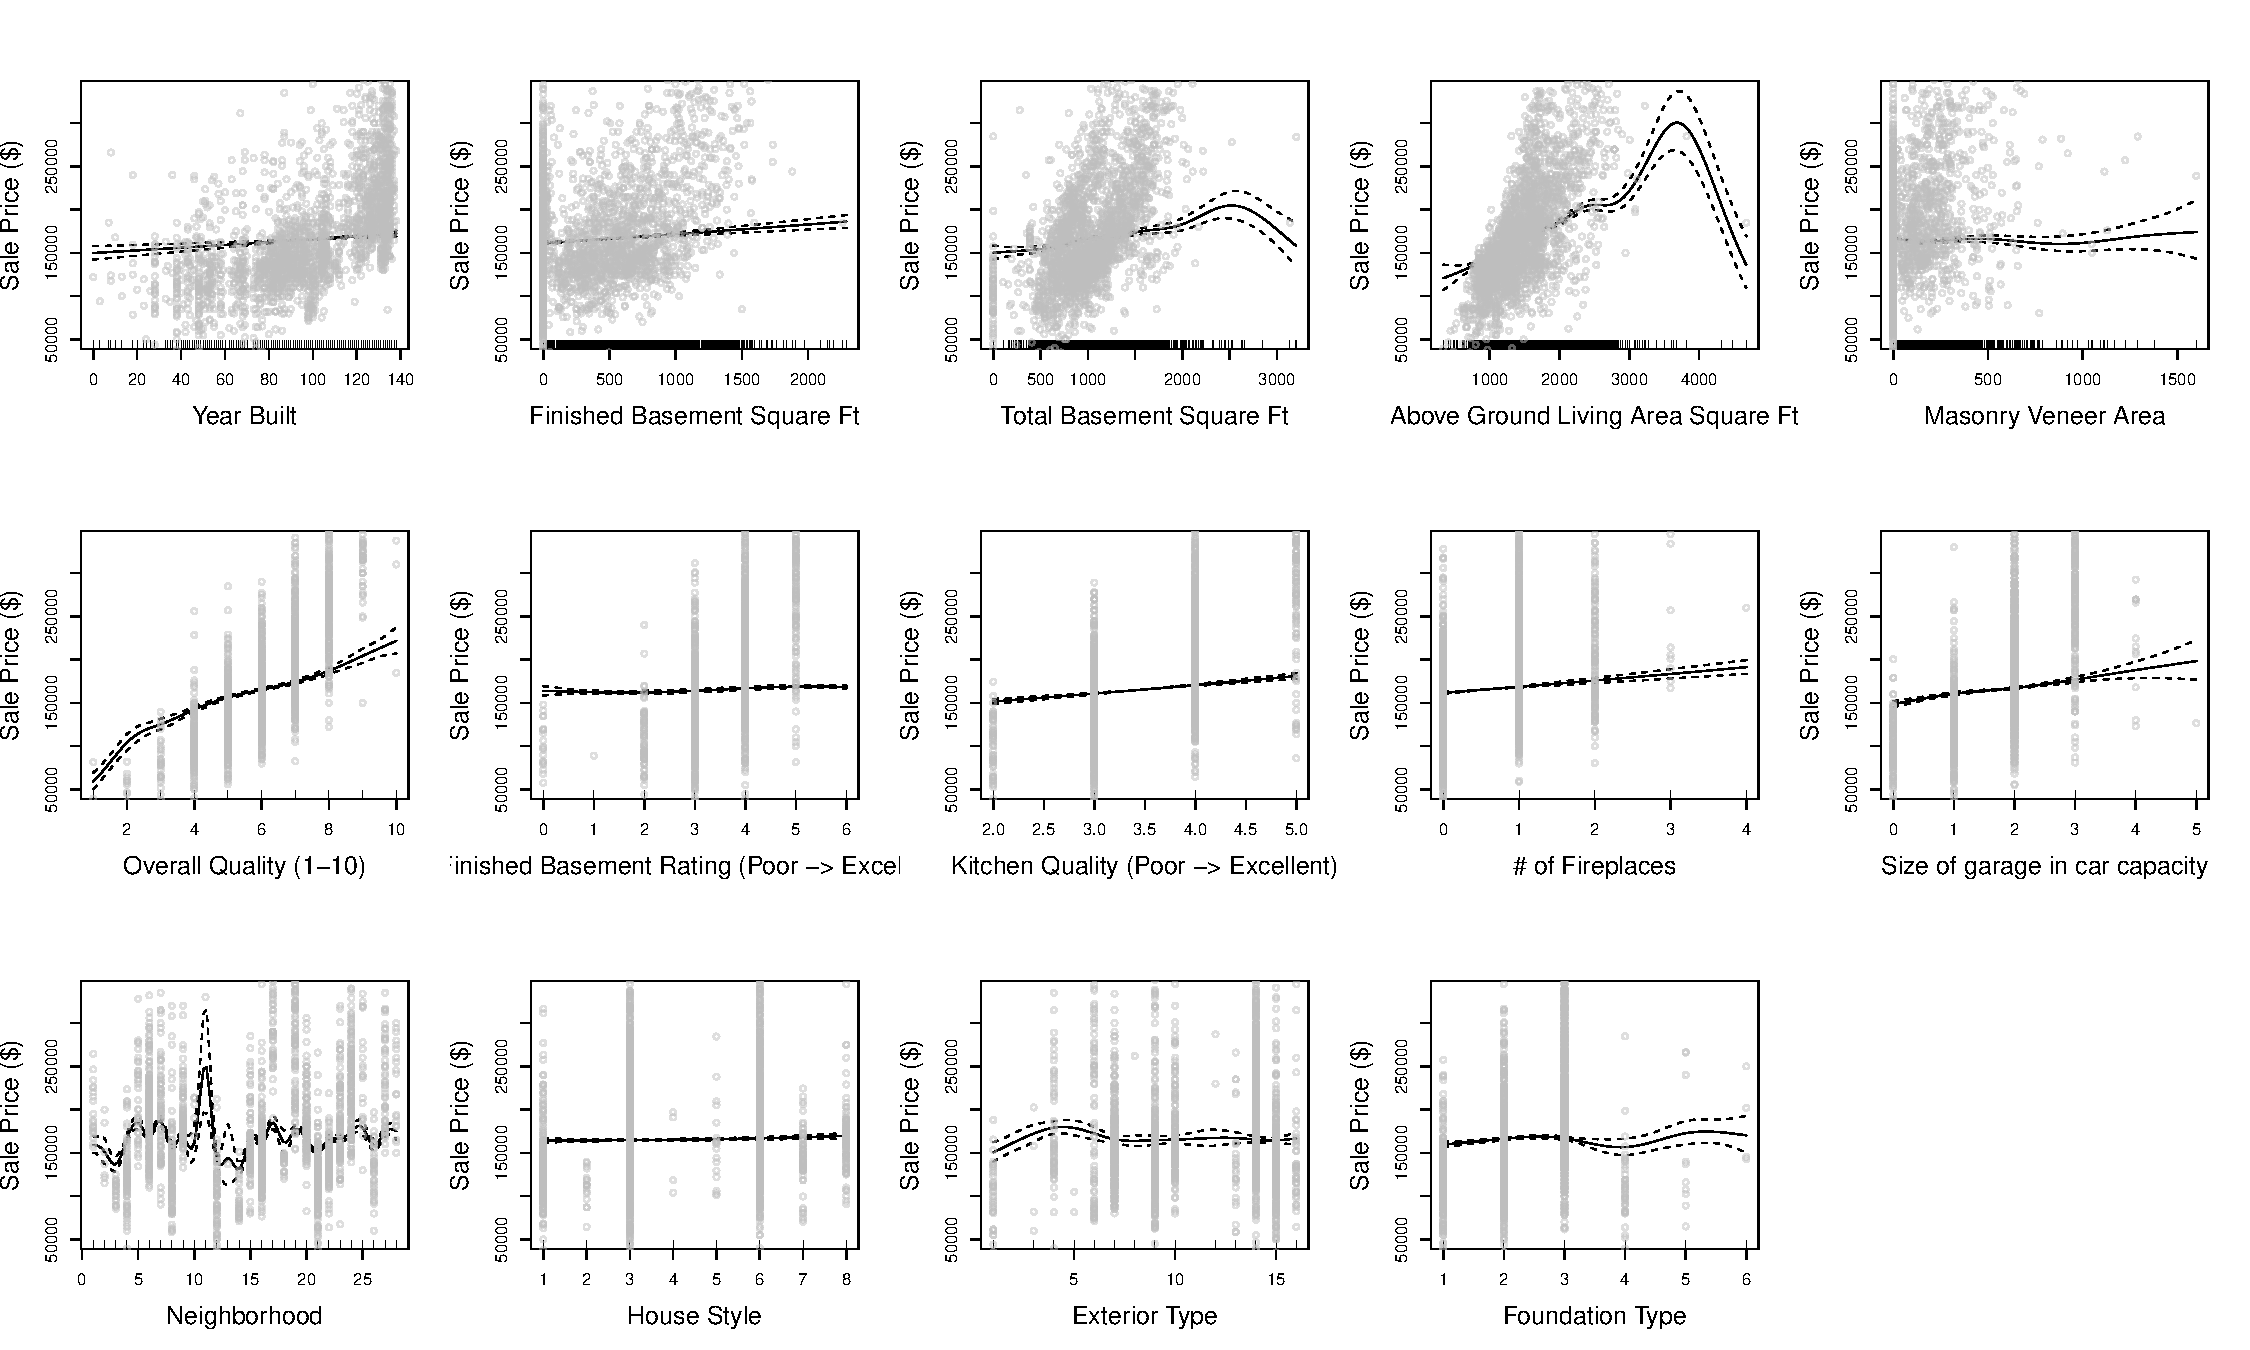
\includegraphics{STAT-444-FINAL-PROJECT-PAPER_files/figure-latex/unnamed-chunk-8-1.pdf}
\caption{Selected smooths plotted against residuals. Row 1 displays
continuous covariates, row 2 displays ordinal/discrete covariates, and
row 3 displays categorical covariates.\label{smooths}}
\end{figure}

We clearly see that there are lots of non-linear trends in several
continuous and ordinal covariates that the GAM handles gracefully. This
is likely why the GAM outperformed the linear regression models, and
best predicted the prices of houses given their characteristics. Since
Lasso, Ridge, and MLR require that the predictors are linear in order to
perform the best, they struggle to fit the least-squares solutions and
see higher RMSE scores. Moreover, Lasso and Ridge approaches only serve
to deal with multicollinearity, not nonlinearity. Ridge shrinks
correlated predictors towards each other, whereas Lasso selects one
correlated predictor and ignores the rest \citep{JSSv033i01}. Since most
of the multicollinearity was addressed in the data preprocessing step,
it makes sense that the MLR, Ridge, and Lasso RMSEs are close to one
another.

\hypertarget{model-assumptions}{%
\subsection{Model Assumptions}\label{model-assumptions}}

The following graphs depict the performance of the final model on the
testing set, fitted using the training set.

\begin{figure}
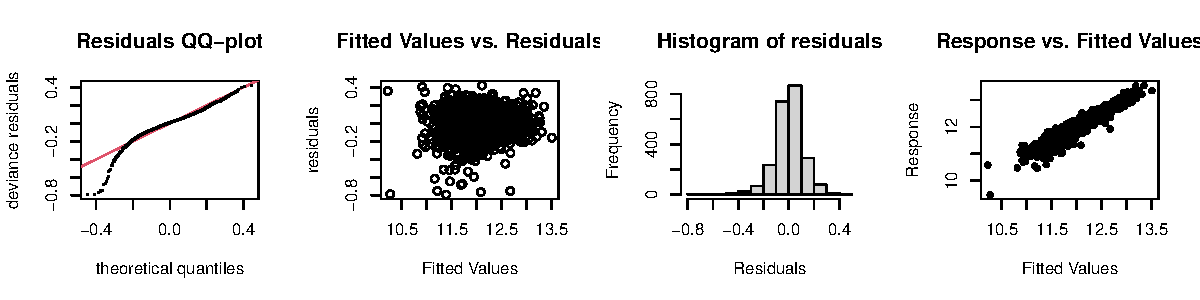
\includegraphics[trim={0 0.4cm 0 0.2cm},clip]{STAT-444-FINAL-PROJECT-PAPER_files/figure-latex/unnamed-chunk-9-1} \caption{Residual QQ-plot, Residual histogram, and Fitted Values vs. Residuals plot\label{assumptions}}\label{fig:unnamed-chunk-9}
\end{figure}

We can see that the normality assumption appears to be violated, as the
tails on the left side of the QQ-plot appear to be quite heavy. Taking a
look at the histogram of residuals, we can see that the model appears to
be undershooting sale prices when the true value is large. This may be
the result of the GAM function smoothing away the wiggliness that might
be required at the tail ends of the sale price values, or outliers in
the data that our preprocessing steps failed to recognize. Thus we have
to be careful when the predicted values lie in the range of the tails of
the sale price values, since we can visually see that there are large
amounts of error at these regions.

\hypertarget{conclusions}{%
\section{Conclusions}\label{conclusions}}

In conclusion, we find that a generalized additive model produced the
best predictions of house sale prices given its physical
characteristics, with a RMSE of \(\$26338.29\), which is acceptable
given the sale price ranges from \(\$12,789\) to \(\$755,000\) with mean
\(\$180,796\) and standard deviation \(\$79,886.69\). This model was
able to correctly capture the non-linearity in the data, and
consistently produce predictions with the lowest RMSE score in both the
cross-validation and testing scenarios. Although there was evidence of
information leak due to the data preprocessing being done before
cross-validation, the GAM still outperformed traditional regression
methods in the test scenario.

One limitation of this analysis was that, in retrospect, of course the
GAM would fit non-linear data better than the linear regression models.
However, the benefit of using a GAM is that much less time and effort
was required to preprocess the data. While are many ways to transform
the covariates such that they are linear with the response and produce
better predicted values under linear models, these methods can be
computationally intensive and sacrifice interpretability. Simply fitting
a GAM allowed a group of undergraduate students to quickly generate
accurate predictions without worrying too much about the usual linear
regression assumptions.

Therefore, given the limited resources our group had to generate these
regression models, the GAM was the best choice for quickly producing
accurate predictions. In the future, it would be worthwhile to compare a
GAM against linear models that better address the nonlinearity, to make
a more fair comparison. It would also be interesting to see how this
model performs on a more recent dataset, as these housing prices are
quite low for today's standards.

\bibliographystyle{imsart-nameyear}
\bibliography{ims.bib}


\end{document}
